Keskitetyn tunnistautumisen lähtökohta on käyttäjän tunnistetietojen poistaminen web-palvelun hallinnasta. Tällöin käyttäjä ei syötä tunnistetietojaan missään vaiheessa web-palveluun, vaan tunnistautuminen tehdään erillisessä tunnistautumispalvelussa. Nykyisin mm. Facebook ja Google tarjoavat julkiset API-rajapinnat, joiden avulla web-palvelut voivat käyttää niitä tunnistautumiseen \cite{facebook}. Tällöin käyttäjä voi kirjautua Internetin palveluihin ilman pelkoa, että hänen tiedot joutuisivat ulkopuolisen käsiin.

Internetissä on lukuisia esimerkkejä palveluista, joissa Facebook-kirjautuminen on käytössä. Kuvassa \ref{facebook_login} on kuvattu kirjautuminen sattumalta valittuun Porkkanamafia-ryhmän WWW-sivulle käyttäen Facebook-kirjautumista. Käyttäjä klikkaa Porkkanamafian WWW-sivulla olevaa ''Login with Facebook'' -nappia, minkä jälkeen käyttäjän selaimeen avautuu Facebook-varmennusikkuna, jossa käyttäjää pyydetään varmentamaan kirjautuminen. Selaimen osoitekenttä osoittaa käyttäjälle, että kirjautuminen tapahtuu nimenomaan Facebook-sivulla (joka on varmennettu SSL-sertifikaatilla), joten käyttäjän Facebook-tun\-nis\-te\-tie\-dot eivät päädy Porkkanamafian haltuun \cite{facebook}. Kirjautuminen tehdään Facebookiin, joten tunnistetiedot pysyvät vain käyttäjän ja Facebookin hallussa.

Kirjautumisen jälkeen käyttäjälle luodaan Porkkanamafian sisäiseen käyttäjätietokantaan rivi, jossa on viittaus hänen Facebook-tunnukseensa. Kun käyttäjä tämän jälkeen palaa sivulle ja kirjautuu sisään jälleen Facebook-tunnuksilla, voidaan hänet yhdistää kannasta löytyvään käyttäjään. Näin palvelu on ulkoistanut tunnistautumisen ulkopuoliselle taholle eikä käyttäjän tarvitse muistaa uusia tunnistetietoja, vaan hän voi käyttää Facebook-kirjautumista myös jatkossa tullessaan Porkkanamafian sivulle.

Samaa periaatetta voidaan käyttää myös organisaatioiden sisäisessä tunnistautumispalvelussa. Tällöin organisaation sisäiseen palvelusuuntautuneeseen arkkitehtuuriin toteutetaan erillinen web-palvelu, joka on yhteydessä organisaation olemassa olevaan käyttäjätietokantaan (esim. LDAP) ja tarjoaa Facebookia vastaavan tunnistautumisen.

\begin{figure}[ht]
\centering
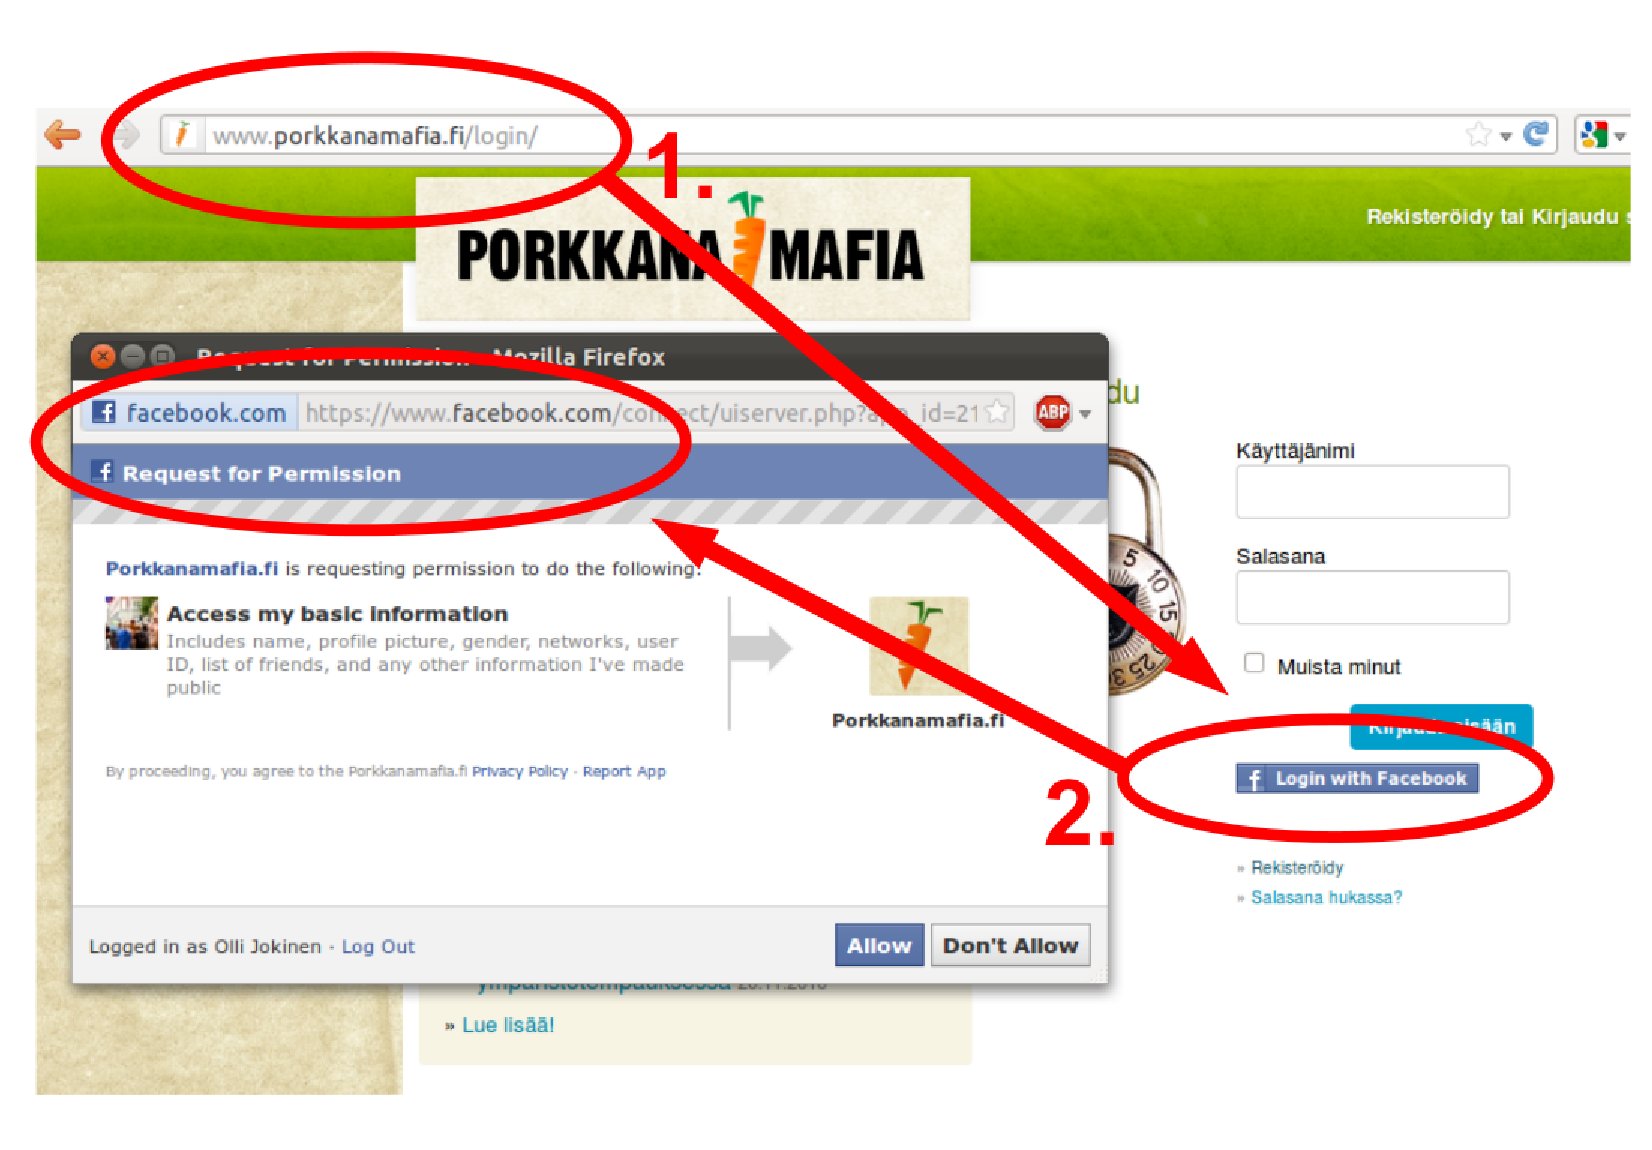
\includegraphics[width=0.7\textwidth]{tunnistautuminen/keskitetty/facebook.eps}
\caption{Käyttäjän kirjautuminen Facebook-tunnuksilla Porkkanamafian web-palveluun.}%
\label{facebook_login}
\end{figure}